\section{Referencial Teórico}
	\label{sec:referencial}
	
%%%%%%%%%%
% Retomada das Definições
%%%%%%%%%%	

Um documento textual, sobre tudo quando longos, são frequentemente um sucessão de tópicos. 
%%%%%%%%%%
% Segmentação
%%%%%%%%%%
A segmentação textual ou segmentação topical é a tarefa de dividir um texto mantendo em cada parte um tópico com seu significado completo.
	
%%%%%%%%%%
% Segmento
%%%%%%%%%%	
Um segmento pode ser visto como uma sucessão de unidades de informação que compartilham um tópico essas unidades podem ser, por exemplo, palavras, sentenças ou parágrafos. Sendo a menor parte de um segmento, portanto são consideradas candidatas a limite entre segmentos.

%%%%%%%%%%
% Coesão léxica como **presuposto básico**
%%%%%%%%%%
Trabalhos anteriores se apoiam na ideia de que a mudança de tópicos em um texto é acompanhada de uma proporcional mudança de vocabulário, essa ideia, chamada de coesão léxica, sugere que a distribuição das palavras é um forte indicador da estrutura do texto. A partir disso, vários algoritmos foram propostos baseados na ideia de que um segmento pode ser identificado e delimitado pela análise das palavras que o compõe~\cite{Galley2003}~\cite{Boguraev2000}.



%, bem como é necessário mensurar suas similaridades. { asunidades de medida}

%%%%%%%%%%
% Porque cosseno
%%%%%%%%%%
Uma vez que a coesão léxica é pressuposto básico da maioria dos algoritmos, o cálculo da similaridade entre unidades de informação (comumente sentenças) é fundamental. Uma medida de similidade frequentemente utilizada é o cosseno, a qual pode ser vista na Equação~\ref{equ:cosine}, sendo $f_{x,j}$ a frequência da palavra $j$ na sentença $x$ e $f_{y,j}$ sendo a frequência da palavra $j$ na sentença $y$.


\begin{equation}
Sim(x,y) = \frac
{\Sigma_j f_{x,j} \times f_{y,j}}
{\sqrt{\Sigma_j f^2_{x,j} \times \Sigma f^2_{y,j}}}
\label{equ:cosine}
\end{equation}


%%%%%%%%%%%%%%%%%%%%%%%%%%%%%%%%%%%%%%%%%%%%%%%
%%%              TextTiling                 %%%
%%%%%%%%%%%%%%%%%%%%%%%%%%%%%%%%%%%%%%%%%%%%%%%

Entre os principais trabalhos da literatura podemos citar o  \textit{TextTiling}~\cite{Hearst1994} e o \textit{C99}~\cite{Choi2000}, os quais são mostrados a seguir.

O \textit{TextTiling} é um algoritmo baseado em janelas deslizantes, onde para cada candidato a limite, analisa-se o texto circundante. Um limite ou quebra de segmento é identificado quando a similaridade entres os blocos apresenta uma queda considerável.

%Ela propõe um algoritmo baseado em janelas deslizante, para analisar blocos de texto adjacentes e identificar os limites com base nas similaridades dos blocos.

O \textit{TextTiling} recebe uma lista de candidatos a limite, usualmente finais de parágrafo ou finais de sentenças. Para cada posição candidata são construídos 2 blocos, um contendo sentenças que a precedem e outro com as que a sucedem. O tamanho desses blocos é um parâmetro a ser fornecido ao algoritmo e determina o tamanho mínimo de um segmento.
%
Em seguida, os blocos de texto são representados por vetores que contém as frequências de suas palavras. Então, usa-se cosseno (Equação~\ref{equ:cosine}) para calcular a similaridade entre os blocos adjacentes a cada candidato e identifica-se uma transição entre tópicos pelos picos na curva se dissimilaridade como apresentado na Figura~\ref{fig:curvadedissimilaridade}.

%sempre que a similaridade cai abaixo de um \textit{threshold}.

O \textit{TextTiling} apresenta baixa complexidade computacional, devido a simplicidade do algoritmo e baixa eficiência quando comparado a outros métodos mais sofisticados como apresentados em~\cite{Choi2000, Kern2009, Misra2009}.



%%%%%%%%%%%%%%%%%%%%%%%%%%%%%%%%%%%%%%%%%%%%%%%
%%%                  C99                    %%%
%%%%%%%%%%%%%%%%%%%%%%%%%%%%%%%%%%%%%%%%%%%%%%%

Choi \cite{Choi2000} apresenta um esquema de ranking em seu algoritmo, o \textit{C99}. 
%
Embora muitos trabalhos utilizem matrizes de similaridades, o autor traz obervações.
%
Ele aponta que para pequenos segmentos, o cálculo de suas similaridades não é confiável, pois uma ocorrência adicional de uma palavra causa um impacto desproporcional no cálculo.
%
Além disso, o estilo da escrita pode não ser constante em todo o texto. Choi sugere que, por exemplo, textos iniciais dedicados a introdução costumam apresentar menor coesão do que trechos dedicados a um tópico específico. 
%

Portanto, comparar a similaridade entre trechos de diferentes regiões, não é apropriado.
% Complexidade O(n²)
Devido a isso, as similaridades não podem ser comparadas em valores absolutos. Então, o autor apresenta um esquema de \textit{rankings} para contornar esse problema.


%

% 1 cria uma matrix de similaridades
% 2 cria a matrix de ranking
% 3 aplica divisive clustering

% mask = quadro
% pegar um exemplo --> mostrar os numeros dentro do quatro e pq o resultado foi aquele

% colocar os passos na imagem


Inicialmente é construída uma matriz que contém as similaridades de todas as unidades de texto. Em seguida, cada valor na matriz de similaridade é substituído por seu ranking local. Onde para cade elemento da matiz, seu \textit{ranking} é o número de elementos vizinhos com valor de similaridade menor ao seu.%, o qual é calculado com a Equação~\ref{equ:ranklocal}. 

Na Figura~\ref{fig:exemplomatrixrank} vemos um quadro de dimensões 3~x~3 destacado na matriz de similaridades, que contém os valores  $\{0,3; 0,4; 0,4; 0,6; 0,5; 0,2; 0,9; 0,5; 0,7\}$, tomando como exemplo o elemento com valor $0,5$, a mesma posição na matriz de \textit{ranks} terá o valor $4$, pois esse é número de vizinhos com valores inferiores a $0,5$ dentro do quadro analisado na matriz de similaridades. 


%nesse exemplo, o valor $0,5$ é substituído por $4$ na matriz de ranks pois há 4 vizinhos com valor inferior

%o valor $0,5$ é comparado com seus elementos vizinhos, o


%Um exemplo é mostrado na Figura \ref{fig:exemplomatrixrank} abaixo, onde utiliza-se uma máscara de largura igual a 3.



  \begin{figure}[!h]

	\centering
	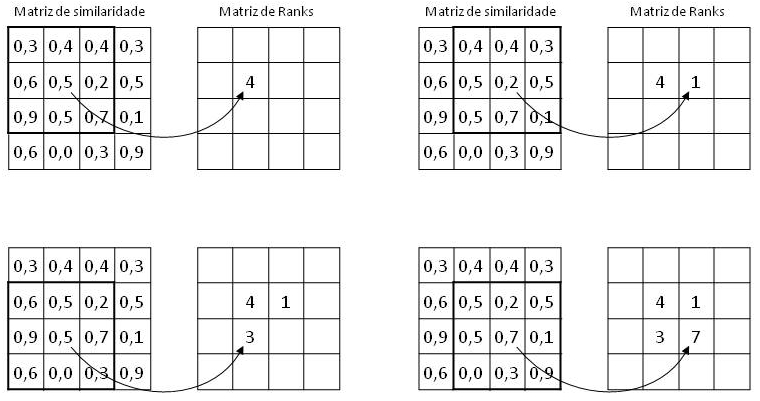
\includegraphics[width=0.45\textwidth]{exemplo-matrix-rank-noborder.jpg}
	\caption{Exemplo de construção de uma matriz de rank.}
	\label{fig:exemplomatrixrank}

  \end{figure}




%\begin{equation}
%r(x,y) = \frac
%{Numero\ de\ elementos\ com\ similaridade\ menor}
%{Numero\ de\ elementos\ examinados}
%\label{equ:ranklocal}
%\end{equation}


% Clustering Reynar maximization
	
Finalmente, utiliza um método de divisão por \textit{clustering} baseado no algoritmo de maximização de Reynar~\cite{Reynar1998} para identificar os limites entre os segmentos. %Essa abordagem apresenta uma redução taxa de erros de 22\% para 10\%. Por outro lado, exige que a quantidade de segmentos seja conhecida.
%Como melhoramento, os autores apresentam posteriormente uma versão do \textit{C99} que utiliza \textit{Latent Semantic Analisys} (LSA) para calcular as similaridades ao invês de cosseno~\cite{Choi2001-LSA}.





%apontam que a coesão léxica é um forte indicador da estrutura do texto, isto é, a mudança de tópicos é acompanhada de uma proporcional mudança de vocabulário. A partir disso, vários algoritmos foram propostos baseados na ideia de que um segmento pode ser identificado e delimitado pela análise das palavras que o compõe~\cite{Galley2003}~\cite{Boguraev2000}.


%Finalmente, os limites são identificados sempre que a similaridade entre blocos adjacentes entre cada candidato ultrapassa um determinado \textit{threshold}.



% Mensionar que existem duas abordagens principais - Baseada em coesão léxiam e em discursos [ver a pg 2 do Text Segmentation With Topic Moeling and Entity Coherence]




%Há ainda outros critérios para segmentação como a segmentação temática 

%outros tipos de abordagem
%	Segmentação funcional
%	Segementação temática
	